\chapter[Gene regulation via histone modifications, nucleosome positioning
and nuclear architecture in \textit{P. falciparum}
]{Multiple dimensions of epigenetic gene regulation in the malaria parasite
\textit{Plasmodium falciparum}}

\graphicspath{{12_plasmodium/}}

\begin{work}

This chapter has been published in a slightly modified form in
\citep{ay:multiple} as a joint work with Ferhat Ay, Evelien Bunnik,
Jean-Philippe Vert, Karine Le Roch and William S. Noble and

\end{work}



\begin{abstract}{Abstract}

\textit{Plasmodium falciparum} is the most deadly human malaria parasite, responsible
for an estimated 207 million cases of disease and 627,000 deaths in 2012.
Recent studies reveal that the parasite actively regulates a large fraction of
its genes throughout its replicative cycle inside human red blood cells and
that epigenetics plays an important role in this precise gene regulation. Here
we discuss recent advances in our understanding of three aspects of epigenetic
regulation in \textit{P. falciparum}: changes in histone modifications, nucleosome
occupancy and the three-dimensional genome structure. We compare these three
aspects of the \textit{P. falciparum} epigenome to those of other eukaryotes, showing
that large-scale compartmentalization is particularly important in determining
histone decomposition and gene regulation in \textit{P. falciparum}. We conclude by
presenting a gene regulation model for \textit{P. falciparum} which combines the
described epigenetic factors and by discussing the implications of this model
for the future of malaria research.

Keywords: malaria, nucleosome occupancy, histone modifications,
three-dimensional genome organization, epigenetics, gene regulation, virulence
genes.
\end{abstract}

Abbreviations: PfEMP1, Plasmodium falciparum Erythrocyte Membrane Protein 1;
var, family of genes that encode PfEMP1 proteins; ApiAP2, a family of
transcription factors in Plasmodium; mRNA, messenger RNA; FISH, fluorescent in
situ hybridization; 3C, chromatin conformation capture; 4C, circularized
chromatin conformation capture; Hi-C, chromatin conformation capture coupled
to next-generation sequencing; ChIA-PET, Chromatin Interaction Analysis by
Paired-End Tag Sequencing; PTM, post-translational modification; TSS,
transcription start site; ChIP, chromatin immunoprecipitation; TAD,
topologically associated domain; H4K20me3, histone H4 lysine 20
trimethylation; H3K9ac, histone H3 lysine 9 acetylation; H3K{N}me3, histone H3
lysine {N} trimethylation; H2A, histone H2A; H2A.Z, H2B.Z, variants of histone
H2A and H2B; SHH, sonic hedgehog gene; Hox, a group of homeobox genes; OR,
olfactory receptors; hpi, hours post invasion.


\section{Introduction}


\begin{figure}
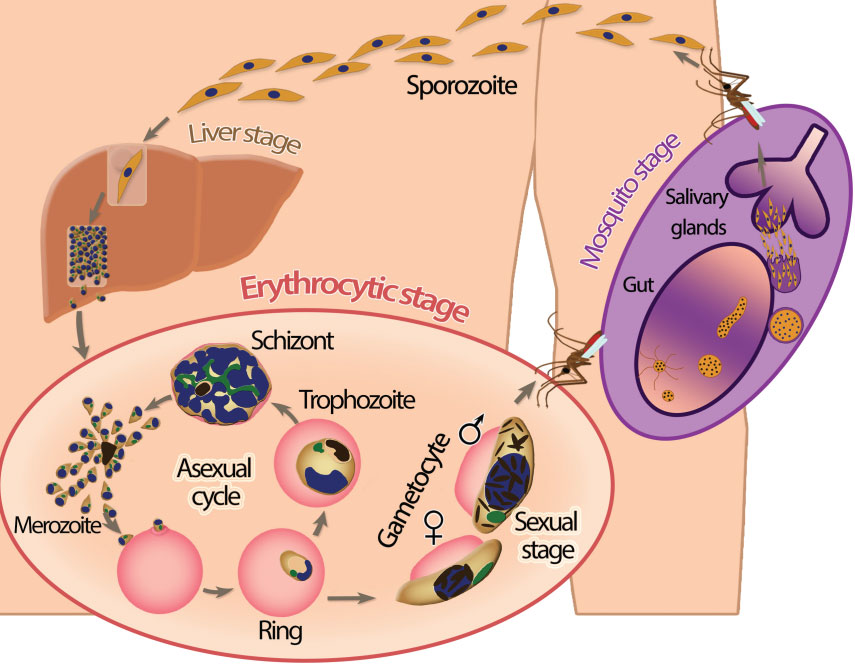
\includegraphics[width=\linewidth]{figures/fig1.png}
\caption{Overview of the {\em P. falciparum}}
\label{fig:overview}
\end{figure}

The complex life cycle of \textit{Plasmodium falciparum} includes multiple stages in
both the human host and the mosquito vector (reviewed in
\citet{greenwood:malaria}) (Fig~\ref{fig:overview}). Human
infection starts with the bite of an infected female Anopheles mosquito,
resulting in the transfer of sporozoites that quickly migrate to the liver.
Inside liver cells (hepatocytes), these sporozoites multiply extensively over
a period of approximately two weeks and are then released into the bloodstream
in the form of thousands of merozoites (Fig.~\ref{fig:overview} - liver stage).
During the next
stage of its life cycle, the parasite replicates in red blood cells
(erythrocytes) by means of an unusual process of cell division called
schizogony. While the parasite progresses through three distinct developmental
stages (ring, trophozoite and schizont), it undergoes multiple rounds of
nuclear replication followed by division of the multinucleated parasite into
16 to 32 daughter merozoites (Fig.~\ref{fig:overview} - asexual cycle).
Upon bursting out of
the host cell, these merozoites are released into the bloodstream and will
invade new erythrocytes. During the asexual cycle, the parasite can commit to
sexual development (reviewed in \citet{baker:malaria}),
resulting in differentiation into a male
or female gametocyte (Fig.~\ref{fig:overview} - sexual stage). The uptake of mature gametocytes
by a feeding mosquito followed by the further development of the parasite in
the mosquito midgut completes the \textit{P. falciparum} life cycle
(Fig.~\ref{fig:overview} - mosquito
stage).

The asexual replication cycle is responsible for symptomatic disease and for
the complications that are associated with severe malaria, such as anemia due
to rupturing of red blood cells. In addition, severe disease can result from
cytoadherence, the attachment of \textit{P. falciparum}-infected erythrocytes to the
smallest blood vessels, preventing clearance by the spleen and causing organ
dysfunction. This cytoadherence is mediated by a family of parasite virulence
proteins that are expressed on the erythrocyte surface, \textit{Plasmodium
falciparum}
Erythrocyte Membrane Protein 1 (PfEMP1) \citep{baruch:cloning, smith:switches,
su:large}. Each \textit{P. falciparum} parasite has
approximately 60 different PfEMP1 variants encoded by var genes, only one of
which is expressed at any time. Switching var gene expression enables the
parasite to escape from host immune responses \citep{bull:parasite,
roberts:rapid}. This process of antigenic
variation is one example of the excellent adaptation of the parasite to
survive in the human host.

The development of \textit{P. falciparum} through the different stages of its life
cycle is thought to be driven by coordinated changes in gene expression. Over
the last decade, it has become clear that the parasite relies on an unusual
combination of regulatory mechanisms for gene expression, and that these
mechanisms are largely dependent on epigenetic processes (reviewed in
\citep{cui:chromatin-mediated, duffy:role, hoeijmakers:placing,
horrocks:control, deitsch:mechanisms, voss:epigenetic}).
In higher eukaryotes, gene expression is often mediated by transcription
factors that bind to cell- or tissue-specific promoters and give rise to the
expression of a subset of genes specific to that cell type or tissue
\citep{dunham:integrated}.
However, despite extensive computational searches, relatively few
transcription factors have been identified in \textit{P. falciparum}
\citep{balaji:discovery, coulson:comparative}, only a
handful of which are known to be specific to a certain stage
\citep{campbell:identification}. A notable
example is PfAP2-G, a member of the ApiAP2 transcription factor family, that
drives expression of gametocyte-specific genes and is crucial for the
development of gametocytes \citep{kafsack:transcriptional, sinha:cascade}.
On the other hand, a relatively large
number of genes are predicted to encode proteins involved in chromatin
structure, mRNA decay and translation rates \citep{coulson:comparative},
suggesting that alternative
mechanisms of gene regulation, at the epigenetic as well as post-translational
levels, may be more important for gene regulation in \textit{P. falciparum.}
Here we focus on three important aspects of epigenetic gene regulation in
\textit{P.
falciparum}, all of which are related to how DNA is packed in the nucleus (see
\citet{chung:post-translational, leroch:genomics, suvorova:transcript,
kramer:rna, bunnik:polysome}
 for articles discussing post-transcriptional regulation and see
 \citet{ponts:genome-wide}
for a discussion on DNA methylation, which is not well-characterized in
\textit{P.
falciparum}). Similar to other eukaryotes, \textit{P. falciparum }packages its DNA in
the form of a condensed DNA-protein complex called chromatin. The basic
packaging unit is a nucleosome, a stretch of approximately 147~bp of DNA
wrapped around a core of eight histone proteins. Several layers of
higher-order compaction of these strings of nucleosomes together create a
highly structured nucleus. The organization of chromatin at both local and
global levels is known to be involved in transcriptional regulation
\citep{jenuwein:translating,zentner:regulation, nora:segmental,
belmont:large-scale}.
Local chromatin structure encompasses two main regulatory processes: the
post-translational modification (PTM) of histone proteins that form
nucleosomes, and nucleosome occupancy, which comprises the location,
frequency, binding strength and protein composition (i.e., variant versus
canonical histones) of nucleosomes on DNA.

At the global level, the organization of chromatin has been studied
extensively, initially using gene-by-gene approaches such as immunofluorescent
microscopy and fluorescent in situ hybridization (FISH) and, more recently,
with chromatin conformation capture (3C)-based next-generation sequencing
assays. 3C-based assays have enabled genome-wide profiling of chromatin
contacts for various organisms including human, mouse, fruit fly, budding
yeast and  \textit{P. falciparum} \citep{ay:three-dimensional,
dixon:topological, duan:three, lemieux:genome-wide,
lieberman-aiden:comprehensive, sexton:three-dimensional}. These profiles have
yielded significant insights into the relation between chromatin organization
and transcription, revealing for example the compartmentalization of the
genome into regions of transcriptionally active euchromatin and
transcriptionally silent heterochromatin. Furthermore, for the haploid
\textit{P. falciparum} genome, the 3D models inferred from these contact
profiles allowed tracking changes in nuclear organization throughout different
stages of the parasite life cycle \citep{ay:three-dimensional}.

In the following sections, we provide an overview of our current understanding
of chromatin organization and its role in transcriptional regulation in
\textit{P. falciparum}. We first describe various characteristics of local
chromatin structure and subsequently focus on three-dimensional genome
architecture. Finally, we combine these local and global views of chromatin to
provide a model that explains our current understanding of the overall nuclear
organization in \textit{P. falciparum} and the role of the epigenome in
regulating gene expression.

\section{Histone modification landscape of the \textit{P. falciparum} genome favors
euchromatin}

\subsection{Post-translational modification of histone proteins}

\begin{figure}
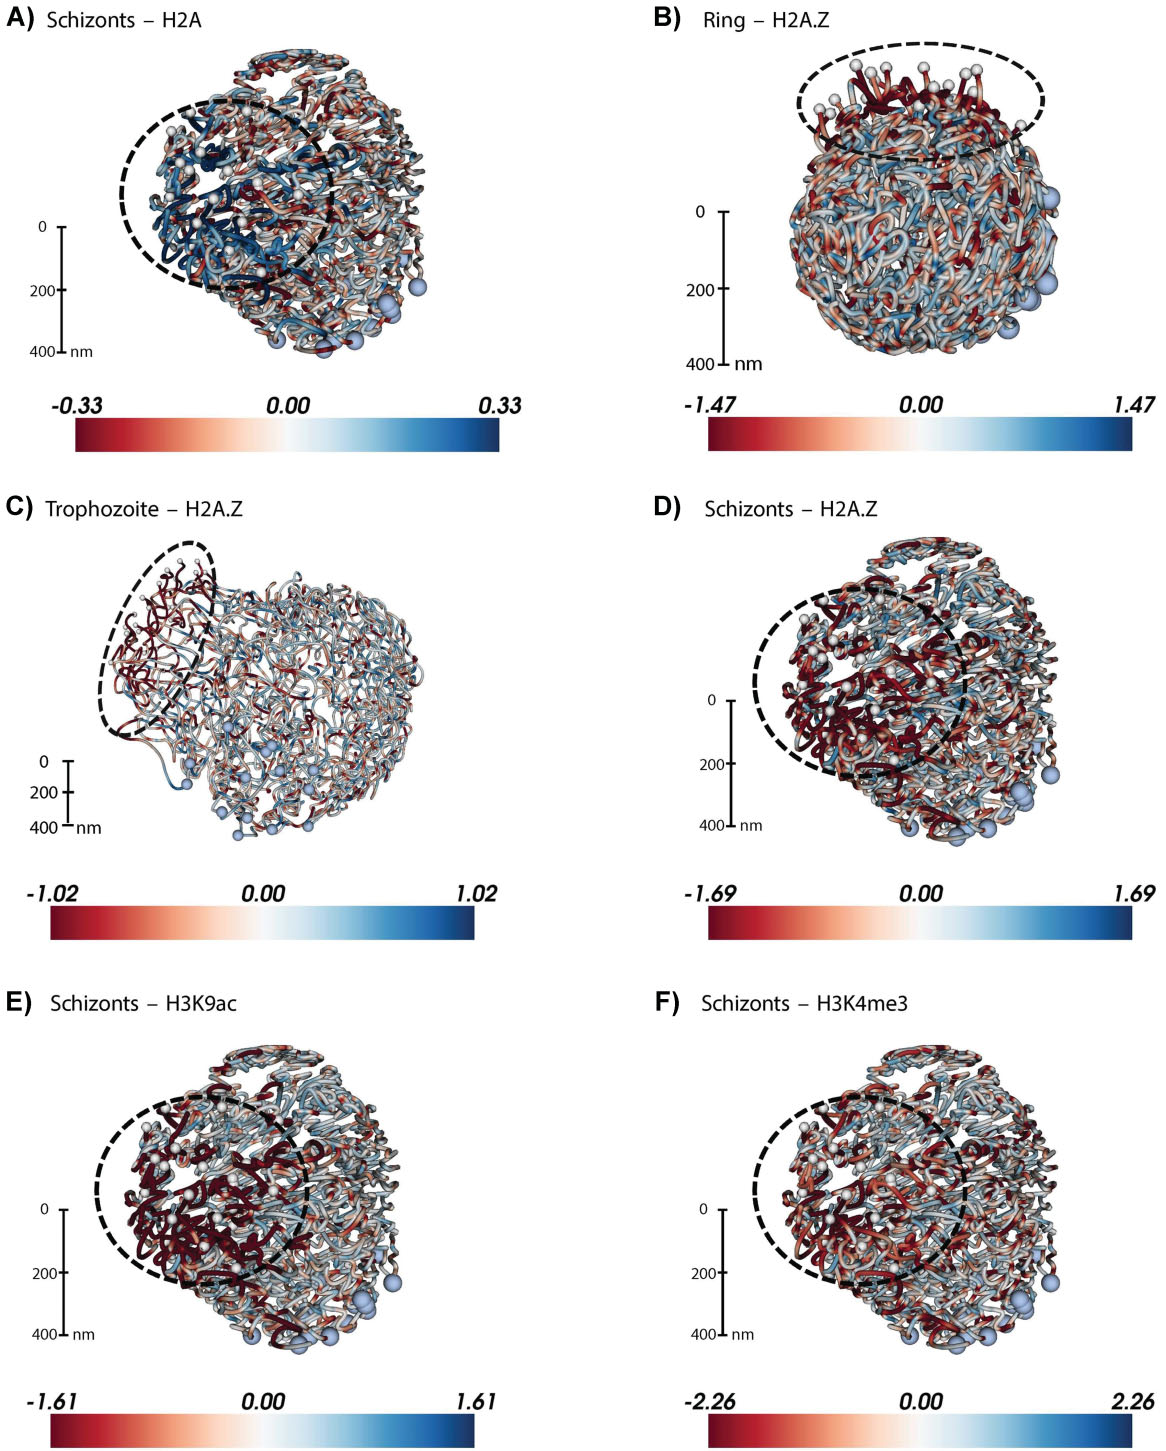
\includegraphics[width=\linewidth]{figures/fig2.png}
\label{fig:3D}
\caption{
Large-scale depletion of the transcriptionally permissive histone variant
H2A.Z and activating histone marks in the telomeric cluster
visualized on the 3D \textit{P. falciparum} genome. ChIP-seq data from Bartfai et al.
\citet{bartfai:h2az} for four histone variants or marks were downloaded from
GEO (accession number: GSE23787) and mapped to the \textit{P. falciparum} genome
(PlasmoDB v9.0) using the short read alignment mode of
BWA (v0.5.9) \citep{li:fast} with default parameter settings.
Reads were post-processed,
and only the reads that map uniquely with a quality score
above 30 and with at most two mismatches were retained for further analysis.
Retained reads were subjected to PCR duplicate elimination
and then were aggregated for each non-overlapping 5~kb bin across the \textit{P.
falciparum} genome. The number of reads for each 5~kb bin was
normalized using the overall sequencing depth of the corresponding ChIP-seq
library. Plotted are the log2 ratios of sequence-depth
normalized number of reads from the ChIP-seq library versus the corresponding
input library (red: depletion, blue: enrichment) for A: H2A at
40 hours post invasion (hpi), B: H2A.Z at 10 hpi, C: H2A.Z at 30 hpi, D: H2A.Z
at 40 hpi, E: H3K9ac at 40 hpi, and F: H3K4me3 at 40 hpi. 3D
models for the ring, trophozoite and schizont stages were generated in
\citet{ay:three-dimensional} and were colored with ChIP-seq enrichment/depletion
from 10, 20, and 40 hpi, respectively. Light blue and white spheres indicate
centromeres and telomeres, respectively. The black dashed circle
denotes the telomeric cluster for each stage. See Supporting information or
http://noble.gs.washington.edu/proj/plasmo-epigenetics for the
rotating 3D figure of each available ChIP-seq library.
}
\end{figure}

Histone proteins consist of a globular core structure and an N-terminal tail
that protrudes from this core domain. Many amino acid residues in the core
domain and in particular in the N-terminal tail can be chemically modified,
with various effects on chromatin organization (Fig.~\ref{fig:3d}). In general, the
addition of an acetyl group neutralizes the positive charge of histone
proteins and thereby disrupts the stability of the DNA-histone interaction.
This destabilization results in a more open chromatin structure and promotes a
transcriptionally permissive state. On the other hand, methylations are
uncharged and do not directly interfere with the interaction between histones
and DNA. Rather, methylations mostly function by recruiting other effector
molecules to the locus, resulting in further modifications of the chromatin.

\subsection{Activating histone marks are abundant and broadly distributed}

In \textit{P. falciparum}, mass spectrometry experiments have identified at
least 50 different histone post-translational modifications (PTMs), including
methylation, acetylation, phosphorylation, ubiquitylation, and sumoylation
\citep{lasonder:insights, miao:malaria, treeck:phosphoproteomes,
trelle:global}. Subsequent chromatin immunoprecipitation (ChIP) studies have
given us insight into the genome-wide distribution of these histone marks in
the asexual cycle (Table 1). In contrast to multicellular eukaryotes, a large
proportion of the genome in \textit{P. falciparum} is constitutively
acetylated \citep{miao:malaria, lopez-rubio:genome-wide}. An abundance of
activating marks has also been observed for other unicellular organisms, such
as \textit{Saccharomyces cerevisiae} and \textit{Tetrahymena thermophila}
\citep{garcia:organismal}. Inhibition of
histone acetyltransferase and deacetylase activity influences the expression
levels of the majority of genes and interferes with parasite growth
\citep{cui:histone, cui:cytotoxic, chaal:histone},
indicative of the importance of acetylation for regulating transcription
levels. Activating marks H3K9ac and H3K4me3 are mainly located in intergenic
regions \citep{bartfai:h2az, jiang:pfsetvs, salcedo-amaya:dynamic}.
Highly transcribed genes carry more H3K9ac marks in their
promoter \citep{bartfai:h2az}, 
and this marking extends into the 5’ coding region
\citep{salcedo-amaya:dynamic}.

\subsection{Repressive histone marks are scarce and localized to specific
regions}

Typical repressive marks, in particular H3K9me3, are almost exclusively found
in repressive clusters containing genes belonging to the virulence families,
such as var, rifin, stevor, and pfmc-2tm \citep{lopez-rubio:genome-wide,
jiang:pfsetvs, chookajorn:epigenetic, lopez-rubio:5}. Interestingly, H3K9me3
is also present at several additional loci, including the gene encoding the
gametocyte-specific transcription factor PfAP2-G
\citep{lopez-rubio:genome-wide} that is tightly
repressed during the asexual cycle. Transcription start sites of silent var
genes are also enriched for H3K36me3 \citep{jiang:pfsetvs},
while this modification is found at
equal levels inside coding regions of active and repressed var genes
\citep{jiang:pfsetvs, ukaegbu:recruitment}.
H3K36me3 is present at lower levels in the rest of the genome and is enriched
at the 3’ end of coding regions of active \textit{P. falciparum} genes, in
agreement with its role in transcriptional elongation in other eukaryotes. The
repressive mark H4K20me3 is also mainly present in var gene clusters, although
its enrichment is not as strong as for H3K9me3 and H3K36me3
\citep{jiang:pfsetvs}. On the other
hand, the single active var gene, out of \~60 family members, is enriched in
active histone marks, such as H3K9ac, H3K4me3, and H4 acetylations
\citep{jiang:pfsetvs, lopez-rubio:5}.
Finally, the repressive mark H3K27me3 has not been detected in the parasite
\citep{trelle:global}, similar to yeast. 
The \textit{P. falciparum} genome organization thus seems
unusual in that a large fraction of its chromatin is continuously in a
transcriptionally permissive state, while the formation of heterochromatin
seems to be limited to virulence and specific sexual genes.

\section{Histone variants and nucleosome occupancy are associated with gene
expression}

\subsection{Plasmodium exhibits a distinctive nucleosome landscape around
coding regions relative to other eukaryotes}

Nucleosome occupancy plays an important role in regulating gene expression by
allowing or restricting access of the transcription machinery to the DNA.
Nucleosomes are not placed uniformly along the genome, but show a distinct
distribution around coding regions \citep{brogaard:map,
buenrostro:quantitative, jansen:nucleosome, lee:high-resolution,
mavrich:nucleosome}. In yeast and higher eukaryotes,
the promoter is characterized by a nucleosome-depleted region, bordered on
either side by strongly positioned -1 and +1 nucleosomes, respectively, both
of which are enriched for the variant histone H2A.Z
\citep{raisner:histone, guillemette:variant, tolstorukov:comparative}. The +1 nucleosome
is located at a fixed distance relative to the transcription start site (TSS),
although this distance varies between organisms \citep{lee:high-resolution}. The +2, +3 and
subsequent nucleosomes form an array of nucleosomes with increasingly more
fuzzy positioning towards the 3’ end of the gene. Finally, the transcription
stop site is again demarcated by a strongly positioned nucleosome, followed by
another nucleosome-depleted region.

Nucleosome organization in \textit{P. falciparum} is similar to other eukaryotes in
several respects. First, the promoter region is depleted of nucleosomes
\citep{bunnik:DNA-encoded, ponts:nucleosome, westenberger:genome-wide}
[59-61], the level of which correlates with transcriptional activity. Second,
highly expressed genes have a more open chromatin organization at their core
promoter than silent genes \citep{bunnik:DNA-encoded, ponts:nucleosome}.
However, the \textit{P. falciparum} nucleosome
landscape also exhibits a number of unusual features. Notably, the TSS is not
marked by a strongly positioned +1 nucleosome; instead, the strongest
nucleosomes are the first and last nucleosomes within the coding region
\citep{bunnik:DNA-encoded, ponts:nucleosome}. Furthermore,
telomeric repeats and subtelomeric regions that contain
the virulence gene families (var, rifin, etc) have higher nucleosome occupancy
levels than the bulk of the genome \citep{bunnik:DNA-encoded,
ponts:nucleosome, segal:genomic}. Intergenic regions, on the
other hand, contain lower nucleosome levels than coding regions
\citep{bunnik:DNA-encoded, ponts:nucleosome, segal:genomic, ponts:nucleosome2},
which is likely to be related to their extremely high AT-content (90-95\%).
AT-rich DNA is inherently inflexible, hampering the winding of DNA around the
histone core \citep{tillo:GC, segal:poly}. 
Finally, intergenic regions in \textit{P. falciparum} are
exclusively occupied by nucleosomes composed of histone variants H2A.Z and
H2B.Z \citep{hoeijmakers:h2az, petter:h2az}, 
which are thought to have adopted a specialized function in \textit{P.
falciparum} to allow nucleosome assembly in these highly AT-rich regions. These
histone variants are thus not restricted to promoter flanking nucleosomes but
have a much broader distribution.

\subsection{Nucleosome dynamics change in concordance with transcriptional
activity during the asexual cycle}

Another unconventional feature of nucleosome organization in \textit{P.
falciparum} is that nucleosome levels vary considerably during the asexual
replication cycle, in parallel with changes in transcriptional activity
\citep{bunnik:DNA-encoded, ponts:nucleosome}.
At the transcriptionally most active trophozoite stage, histone
levels decrease by approximately two-fold 
\citep{bunnik:DNA-encoded, ponts:nucleosome}. This nucleosome depletion
occurs in a genome-wide fashion and is not restricted to genes that are
expressed in the trophozoite stage. As the asexual cycle progresses into the
schizont stage, nucleosomes are re-assembled, resulting in condensation of DNA
as the parasites prepare for egress and re-invasion of a new red blood cell.
Given the correlation between nucleosome density in promoter regions and gene
expression levels, the dynamic nucleosome landscape in \textit{P. falciparum} may have
evolved to compensate for a paucity of specific transcription factors.
Interestingly, \textit{Trypanosoma brucei}, a parasite causing sleeping sickness in
humans, has also developed an unusual nucleosome landscape, where certain
combinations of canonical and variant histones mark the transcription
initiation and termination sites in its genome \citep{siegel:four}.
Reminiscent of the lack
of transcription factors in \textit{P. falciparum}, transcription factors have remained
elusive in \textit{T. brucei}, indicating that these parasites may have followed
parallel evolutionary pathways towards the use of the nucleosome landscape as
a mechanism to regulate gene expression.


\section{Three-dimensional conformation of the \textit{P. falciparum} genome}

\subsection{Principles of nuclear organization in \textit{P. falciparum}}

It has been long known that the eukaryotic nucleus is a highly structured
entity. In addition to three-dimensional conformation of the
chromatin-packaged DNA, key structural landmarks include the nuclear envelope,
nuclear pores and nucleoli. For decades, various microscopic imaging
techniques have been the “go-to” tools for understanding nuclear organization
and chromatin architecture in many different organisms
\citep{cremer:chromosome, misteli:beyond, takizawa:meaning}
[69-71]. In \textit{P.
falciparum}, FISH applications have been instrumental in demonstrating
important characteristics of genome organization in the parasite. In
particular, silent var genes were shown to colocalize with each other near the
nuclear periphery, while the single active var gene is located elsewhere

\citep{lopez-rubio:genome-wide, freitas-junior:frequent, ralph:antigenic}.
Together with the other epigenetic mechanisms outlined above —
histone modifications, histone variants and nucleosome occupancy — the
non-random organization of DNA into repressive centers is believed to play a
crucial role in the one-at-a-time expression of 60 genes in the var family.
Another intriguing discovery from FISH experiments was that the ribosomal DNA
loci that are distributed in a seemingly random fashion on different \textit{P.
falciparum} chromosomes show non-random colocalization in 3D
\citep{mancio-silva:clustering}. A more
recent study employed several ultrastructural microscopy techniques to study
the distribution of nuclear pore complexes and chromatin throughout the
\textit{P.
falciparum} asexual cycle \citep{weiner:3d}, demonstrating a striking increase in pore
density during the transcriptionally active trophozoite stage, as well as
chromatin decomposition near the nuclear envelope. These changes parallel
previously observed changes in transcriptional activity and nucleosome
occupancy that have been discussed above \citep{ponts:nucleosome}.

\subsection{Profiling of eukaryotic genome architecture using next-generation
sequencing applications}

Within the last decade, the field of genome architecture has been
revolutionized by breakthroughs in combining next generation sequencing with
molecular assays that measure proximities of DNA regions to certain nuclear
landmarks (e.g., lamina, nucleolus) or to other regions in cis or trans (e.g.,
4C, Hi-C, ChIA-PET) \citep{duan:three-dimensional,
lieberman-aiden:comprehensive, fullwood:oestrogen-receptor-alpha-bound,
guelen:domain, koningsbruggen:high-resolution, vogel:detection,
zhao:circular} (see \citep{steensel:genomics} for review).
Applications of these
techniques to multiple genomes including human and mouse have revealed the
organizational hallmarks of genome architecture. These include localization of
gene-rich regions near the nuclear center and heterochromatin near the nuclear
lamina \citep{guelen:domain}, colocalization of ribosomal DNA loci near
nucleoli \citep{koningsbruggen:high-resolution}, and
megabase-scale open/closed chromatin compartments
\citep{lieberman-aiden:comprehensive}. In addition, genomes
of higher eukaryotes are partitioned into megabase-sized topologically
associated domains (TADs) that are enriched for interactions within but not
across domains and are separated from each other by insulator proteins
\citep{dixon:topological, nora:spatial, sofueva:cohesin-mediated}
(see \citep{nora:segmental} 
for review). Finally, these studies have provided us with
examples of cell type-specific chromatin loops bringing distal regulatory
elements in close 3D proximity. Long-range chromatin loops that play
regulatory roles in gene expression include Hox cluster silencing
\citep{ferraiuolo:three-dimensional, rousseau:hox},
control of SHH gene by an enhancer that is located 1~Mb away in human
\citep{li:extensive} [86] and
a validated set of cell type-specific enhancers in mouse \citep{shen:map}.

\subsection{Profiling of \textit{P. falciparum} genome architecture during the asexual
cycle}

As is the case for many other next generation sequencing-based assays,
application of these genome architecture assays has been challenging for the
AT-rich genome of \textit{P. falciparum}. However, within the last year, two groups
have published their results using Hi-C, one profiling the genome architecture
of different \textit{P. falciparum} strains \citep{lemieux:genome-wide} 
and the other modeling the 3D
structure of \textit{P. falciparum}-3D7 at three key stages during its asexual
replication cycle within human red blood cells \citep{ay:three-dimensional}.
These studies revealed
key characteristics of \textit{P. falciparum} genome structure (Table 2), including
colocalization of centromeres, colocalization of telomeres near the nuclear
periphery, colocalization of both internal and subtelomeric virulence gene
clusters near the telomeres, colocalization of rDNA loci that are active in
ring stage parasites and maintenance of chromosomes territories (see
\citet{ay:three-dimensional} for details). Furthermore, Hi-C profiles from
\citet{ay:three-dimensional} exhibit different
polymer behavior in the most transcriptionally active trophozoite stage
compared to the other two stages, suggesting a link between overall chromatin
compaction and transcriptional activity. The degree of telomere colocalization
and the repressive effect of the telomeric compartment is also most pronounced
in this trophozoite stage, suggesting a strict compartmentalization to
segregate genes that need to be repressed from the rest. Finally, both the
Hi-C contact maps and the 3D models inferred from them suggest a tight
correlation between the 3D location of a gene and its expression. Gene pairs
located nearby in 3D have significantly higher expression correlation compared
to other pairs, even after discarding intra-chromosomal pairs that would be
biased by their genomic distance in 1D \citep{ay:three-dimensional}. Overall, these observations
suggest that \textit{P. falciparum} chromatin is highly structured at the large scale
and that this structure provides a potential epigenetic mechanism to regulate
gene expression.

The folded chromosome structure seen in \textit{P. falciparum} is similar to what has
been observed in budding and fission yeast \citep{duan:three,
tanizawa:mapping}. However, chromosome
looping to achieve localization of var genes in repressive perinuclear
compartments results in a more complex three-dimensional organization of the
\textit{P. falciparum} genome compared to yeast, even though these organisms have
similarly sized genomes \citep{ay:three-dimensional}.
Interestingly, the clonal var gene expression
and clustering of all remaining var genes in repressive heterochromatin is
strikingly similar to the epigenetic signature of the ~1,400 olfactory
receptor genes in the mouse, all except one of which are located in
heterochromatic foci enriched for H3K9me3 and H4K20me3, resulting in monogenic
and monoallelic expression \citep{magklara:epigenetic, lyons:epigenetic}.
In comparison to higher eukaryotes, such
as human, mouse and fly, the \textit{P. falciparum} genome organization is relatively
simple and does not display TADs. The nuclear architecture in \textit{P.
falciparum}
thus exploits features from both unicellular and multicellular organisms.

\section{A combined model of epigenetic gene regulation in \textit{P.
falciparum}}

\subsection{Nuclear organization and gene regulation}

The epigenetic makeup of the \textit{P. falciparum} genome, as outlined above, points
towards a binary nuclear organization, with the majority of the genome present
in the form of euchromatin, while a limited number of genes are organized into
strongly repressed heterochromatin. This heterochromatin is localized at the
nuclear periphery and is characterized by high nucleosome density (Fig. 2A),
the presence of repressive histone marks H3K9me3, H3K36me3 and H4K20me3 (Fig.
3A-C), and the absence of the transcription-associated histone variant H2A.Z
(Fig. 2B-D) and histone marks H3K9ac (Fig. 2E) and H3K4me3 (Fig. 2F and 3D).
It was recently demonstrated that heterochromatin protein 1 (HP1) and \textit{P.
falciparum} histone deacetylase 2 (PfHda2) are both essential for maintaining
heterochromatic regions \citep{brancucci:heterochromatin, coleman:plasmodium}.
Depletion of either HP1 or PfHda2 resulted in
an arrest of parasite development at the trophozoite stage and a loss of var
gene repression. In addition, an increase in the number of parasites
differentiating into gametocytes was observed, indicating that the gametocyte
transcription factor locus pfap2-g is also under strict epigenetic control.
The remaining euchromatic fraction of the genome has several notable features,
including perinuclear compartments containing the active var gene or active
rDNA genes (Fig. 4A). In addition, clustering of silent genes that are
specific to other stages of the parasite’s life cycle
\citep{ay:three-dimensional}, suggests the
presence of small heterochromatic islands, as observed at the trophozoite
stage by advanced transmission and scanning electron microscopy
\citep{weiner:3d}.

\subsection{Remodeling of the nuclear organization during the asexual cycle}

Microarray and RNA-seq studies have shown that 70-80\% of all genes are
expressed in the asexual replication cycle, in particular during the
trophozoite stage \citep{bunnik:polysome, leroch:discovery, otto:new}.
During the 48-hour cycle, the nucleus and
chromatin are dramatically remodeled to facilitate this high transcriptional
activity (Fig. 4B and Table 2). First, the nucleus expands in size
\citep{weiner:3d}, which
can also be readily observed in microscopy images of Giemsa stained parasites
\citep{ay:three-dimensional}. Second, the number of nuclear pores increases 
drastically, from 3-7
clustered pores in the ring stage to 12-58 pores that are uniformly
distributed around the nucleus in the trophozoite stage \citep{weiner:3d}.
Third, in line
with the increased nuclear volume, the chromatin opens up
\citep{ay:three-dimensional, weiner:3d}, accompanied
by removal of nucleosomes \citep{bunnik:DNA-encoded, ponts:nucleosome}
 and increased intermingling of chromosomes
\citep{ay:three-dimensional}. Despite these large-scale nuclear dynamics, the centromeres, telomeres
and repressed var genes remain clustered. The correlation of nucleosome
density of gene promoters with transcriptional activity of individual genes
suggests that local chromatin organization may play an important role in
regulating the level of gene expression \citep{bunnik:DNA-encoded}. The transitioning of the
parasite from the trophozoite stage to the schizont stage is characterized by
a reversion of nuclear changes, including reassembly of nucleosomes and
re-establishment of chromosomal territories, which results in recompaction of
the genome. Finally, during DNA replication, the nucleus divides into multiple
small daughter nuclei, each with a small number of the nuclear pores that were
present in the original nucleus \citep{weiner:3d}.

\section{Outstanding questions}

\subsection{Clustering of repressive heterochromatin}

Whether heterochromatin containing silent var genes is organized into a single
large repressive center or is divided over a small number of perinuclear foci
remains a topic of debate. FISH images visualizing the location of
telomere-associated repeat elements or var gene promoters typically show 2-6
foci distributed around the nucleus \citep{lopez-rubio:genome-wide,
freitas-junior:frequent, ralph:antigenic, voss:var}. On the other hand, single
foci were observed by immunofluorescence microscopy for H3K9me3, H3K36me3, and
heterochromatin protein 1 \citep{ukaegbu:recruitment, dahan:pfsec13},
all of which are strongly associated with
the repressed var genes. In addition, the Hi-C-derived three-dimensional
models of the \textit{P. falciparum} genome showed strong clustering of centromeres and
telomeres \citep{ay:three-dimensional} (Fig. 4A), a
chromosome configuration that has been observed in
other organisms \citep{duan:three-dimensional, tanizawa:mapping,
umbarger:three-dimensional}. These models suggested the organization of
subtelomeric var genes into a single cluster at the nuclear perimeter. Such
organization, even though seemingly contradicting the FISH data, may be due to
aggregation across a large population of cells for Hi-C experiments. If each
var gene cluster is randomly located in one of multiple repressive clusters in
each cell, then the aggregate signal would suggest colocalization of all var
genes. However, it may conceivably be beneficial to locate all repressed genes
in close proximity of each other to regulate the expression of a single var
gene and the tight repression of all remaining family members. Additional
experiments will be necessary to unravel the precise mechanisms by which var
gene expression is controlled, by further dissecting the effect of gene
localization, nuclear architecture, and gene-to-gene communication on this
process. In particular, Hi-C experiments on single cells would likely provide
significant insight into the localization of active and repressed var genes,
as well as the extent of cell-to-cell variability. 

\subsection{Mediators of epigenetic control and nuclear remodeling}

Drastic remodeling of the nucleus and chromatin are likely to be driving
forces behind the wave of transcriptional activity during the trophozoite
stage. Components involved in these dynamic processes may thus be promising
targets for antimalarial drugs. Future research should therefore focus on
understanding the molecular mechanisms involved in chromatin and nuclear
remodeling. For example, very little is known about proteins and enzymes that
regulate the formation of heterochromatin and the global nuclear architecture,
with the exception of the role of HP1 in maintaining repressive perinuclear
chromatin containing the var genes and the pfap2-g locus. A multitude of such
proteins has been identified in other organisms, most notably RNA polymerase
III-associated factor (TFIIIC), cohesin and CCCTC binding factor (CTCF)
(reviewed in \citep{gomez-diaz:architectural}), and are likely 
to have homologues in \textit{P.
falciparum}. Other
potential drug targets include key components involved in expansion of the
nuclear membrane and chromatin remodeling enzymes that regulate the global
nucleosome eviction and re-assembly during the trophozoite and schizont
stages. Analysis of chromatin-associated proteins by proteomics-based
approaches will likely identify many candidates that may be involved in these
processes. In addition, the application of novel genetic engineering tools in
\textit{P. falciparum}, such as the CRISPR/Cas9 system \citep{ghorbal:genome,
zhang:efficient, wagner:efficient}, may enable us to study
the effect of gene deletion or translocation on genome structure to better
understand the determinants of nuclear architecture.

\subsection{Epigenetic control in other parasite stages}
The epigenetic regulation model we present here is based on profiles taken
during the asexual replication cycle. During this phase of the parasite’s life
cycle, the genome seems to be largely shaped by the strict one-at-a-time
expression of the var genes. The absence of var gene expression in all other
parasite stages may have a large impact on chromatin organization. In
addition, while some genes may be constitutively expressed during the
parasite’s life cycle, others may be silenced or activated in these
alternative and highly variable stages, ranging from the male and female
gametocyte, via the diploid zygote in the mosquito midgut, to the haploid
sporozoite. Therefore, we expect generating genome-wide profiles of histone
modifications, nucleosome landscape and three-dimensional architecture during
these other parasite stages to be of great interest to further explore the
epigenetic regulatory mechanisms in \textit{P. falciparum}. 

Furthermore, we know very little about the role of epigenetic control in
transcriptional regulation in other Plasmodium species. \textit{P. vivax}, for example,
has a much lower AT-content (on average 57\%), which is likely to influence the
binding kinetics and preferences of nucleosomes. In addition, \textit{P.
vivax}
expresses a large proportion of its gene family encoding for variant surface
proteins (vir) during the blood stage \citep{bozdech:transcriptome,
fernandez-becerra:variant} [102,103]. The absence of clonal
expression as seen for the var family in \textit{P. falciparum} may relieve the
requirements for strictly repressive heterochromatin in \textit{P. vivax}. Determining
the nucleosome landscape, the location of histone modifications and the
three-dimensional structure of the \textit{P. vivax} genome will therefore also be
extremely informative for our understanding of epigenetic gene regulation.


\section{Conclusions and prospects}
An increasing amount of data highlights the importance of epigenetic
mechanisms in regulating gene expression in \textit{P. falciparum} and other
eukaryotes, including human and mouse \citep{ay:three-dimensional,
dixon:topological, duan:three-dimensional, lemieux:genome-wide,
lieberman-aiden:comprehensive, sexton:three-dimensional}.
Here we have discussed multiple
layers of epigenetic control, including histone modifications, nucleosome
occupancy, histone variants and genome architecture, which are involved in the
precise gene regulation during the asexual replication cycle of the malaria
parasite, \textit{P. falciparum}. We summarized the current understanding of the
interplay among these different layers and how these layers shape the overall
nuclear organization and connect to overall transcriptional activity and to
the one-at-a-time expression of var genes.

Better characterization of epigenetic regulation in \textit{P. falciparum} will
stimulate interest in several exciting directions in malaria research. Further
studies into the establishment and maintenance of strong repressive
compartments in the nucleus may reveal the underlying regulatory mechanisms
and lead to the identification of proteins involved in this process.
Disrupting the function of proteins responsible for maintaining
heterochromatin, such as HP1 \citep{brancucci:heterochromatin},
could be an effective strategy to block
parasite replication during the asexual cycle. Another important event in the
malaria life cycle is gametocytogenesis, which was recently shown to be driven
by the transcription factor PfAP2-G \citep{kafsack:transcriptional,
sinha:cascade}. It would be interesting to fully
characterize the epigenetic factors, such as genome architecture, that help
PfAP2-G target and regulate gametocyte-specific genes. In addition to layers
of epigenetic regulation we focused on here, post-transcriptional and
translational controls are likely to be involved in the timing of protein
expression \citep{suvorova:transcript, kramer:rna, bunnik:polysome, leroch:global}.
Increased insight into these regulatory processes
would significantly advance our understanding of parasite biology and could
mark a major breakthrough in our fight against malaria.


Acknowledgements

The authors have declared no conflict of interest.
This study was financially supported by a Computing Research Association
CIFellows award (NSF award CIF 1136996 to FA), the Human Frontier Science
Program (grant LT000507/2011-L to EMB), the National Institutes of Health
(grants R01 AI85077-04 to KLR and R01 AI106775-02 to WSN/KLR), the European
Research Council (grant SMAC-ERC-280032 to JPV), the European Commission
(grant HEALTH-F5-2012-305626 to JPV/NV) and the French National Research
Agency (grant ANR-11-BINF-0001 to JPV/NV).

References
1 Greenwood BM, Fidock DA, Kyle DE, Kappe SH, et al. 2008. Malaria: progress,
perils, and prospects for eradication. The Journal of clinical investigation
118: 1266-76.
2 Baker DA. 2010. Malaria gametocytogenesis. Mol Biochem Parasitol 172: 57-65.
3 Baruch DI, Pasloske BL, Singh HB, Bi X, et al. 1995. Cloning the P.
falciparum gene encoding PfEMP1, a malarial variant antigen and adherence
receptor on the surface of parasitized human erythrocytes. Cell 82: 77-87.
4 Smith JD, Chitnis CE, Craig AG, Roberts DJ, et al. 1995. Switches in
expression of Plasmodium falciparum var genes correlate with changes in
antigenic and cytoadherent phenotypes of infected erythrocytes. Cell 82:
101-10.
5 Su XZ, Heatwole VM, Wertheimer SP, Guinet F, et al. 1995. The large diverse
gene family var encodes proteins involved in cytoadherence and antigenic
variation of Plasmodium falciparum-infected erythrocytes. Cell 82: 89-100.
6 Bull PC, Lowe BS, Kortok M, Molyneux CS, et al. 1998. Parasite antigens on
the infected red cell surface are targets for naturally acquired immunity to
malaria. Nat Med 4: 358-60.
7 Roberts DJ, Craig AG, Berendt AR, Pinches R, et al. 1992. Rapid switching to
multiple antigenic and adhesive phenotypes in malaria. Nature 357: 689-92.
8 Cui L, Miao J. 2010. Chromatin-mediated epigenetic regulation in the malaria
parasite Plasmodium falciparum. Eukaryot Cell 9: 1138-49.
9 Duffy MF, Selvarajah SA, Josling GA, Petter M. 2012. The role of chromatin
in Plasmodium gene expression. Cell Microbiol 14: 819-28.
10  Hoeijmakers WA, Stunnenberg HG, Bartfai R. 2012. Placing the Plasmodium
falciparum epigenome on the map. Trends Parasitol 28: 486-95.
11  Horrocks P, Wong E, Russell K, Emes RD. 2009. Control of gene expression
in Plasmodium falciparum - ten years on. Mol Biochem Parasitol 164: 9-25.
12  Deitsch K, Duraisingh M, Dzikowski R, Gunasekera A, et al. 2007.
Mechanisms of gene regulation in Plasmodium. The American journal of tropical
medicine and hygiene 77: 201-8.
13  Voss TS, Bozdech Z, Bartfai R. 2014. Epigenetic memory takes center stage
in the survival strategy of malaria parasites. Curr Opin Microbiol 20: 88-95.
14  Consortium EP. 2012. An integrated encyclopedia of DNA elements in the
human genome. Nature 489: 57-74.
15  Balaji S, Babu MM, Iyer LM, Aravind L. 2005. Discovery of the principal
specific transcription factors of Apicomplexa and their implication for the
evolution of the AP2-integrase DNA binding domains. Nucleic Acids Res 33:
3994-4006.
16  Coulson RM, Hall N, Ouzounis CA. 2004. Comparative genomics of
transcriptional control in the human malaria parasite Plasmodium falciparum.
Genome Res 14: 1548-54.
17  Campbell TL, De Silva EK, Olszewski KL, Elemento O, et al. 2010.
Identification and genome-wide prediction of DNA binding specificities for the
ApiAP2 family of regulators from the malaria parasite. PLoS Pathog 6:
e1001165.
18  Kafsack BF, Rovira-Graells N, Clark TG, Bancells C, et al. 2014. A
transcriptional switch underlies commitment to sexual development in malaria
parasites. Nature 507: 248-52.
19  Sinha A, Hughes KR, Modrzynska KK, Otto TD, et al. 2014. A cascade of
DNA-binding proteins for sexual commitment and development in Plasmodium.
Nature 507: 253-7.
20  Chung DW, Ponts N, Cervantes S, Le Roch KG. 2009. Post-translational
modifications in Plasmodium: more than you think! Mol Biochem Parasitol 168:
123-34.
21  Le Roch KG, Chung DW, Ponts N. 2012. Genomics and integrated systems
biology in Plasmodium falciparum: a path to malaria control and eradication.
Parasite Immunol 34: 50-60.
22  Suvorova ES, White MW. 2014. Transcript maturation in apicomplexan
parasites. Curr Opin Microbiol 20C: 82-7.
23  Kramer S. 2014. RNA in development: how ribonucleoprotein granules
regulate the life cycles of pathogenic protozoa. Wiley interdisciplinary
reviews RNA 5: 263-84.
24  Bunnik EM, Chung DW, Hamilton M, Ponts N, et al. 2013. Polysome profiling
reveals translational control of gene expression in the human malaria parasite
Plasmodium falciparum. Genome Biol 14: R128.
25  Ponts N, Fu L, Harris EY, Zhang J, et al. 2013. Genome-wide mapping of DNA
methylation in the human malaria parasite Plasmodium falciparum. Cell host \&
microbe 14: 696-706.
26  Jenuwein T, Allis CD. 2001. Translating the histone code. Science 293:
1074-80.
27  Zentner GE, Henikoff S. 2013. Regulation of nucleosome dynamics by histone
modifications. Nat Struct Mol Biol 20: 259-66.
28  Nora EP, Dekker J, Heard E. 2013. Segmental folding of chromosomes: a
basis for structural and regulatory chromosomal neighborhoods? Bioessays 35:
818-28.
29  Belmont AS. 2014. Large-scale chromatin organization: the good, the
surprising, and the still perplexing. Curr Opin Cell Biol 26: 69-78.
30  Ay F, Bunnik EM, Varoquaux N, Bol SM, et al. 2014. Three-dimensional
modeling of the P. falciparum genome during the erythrocytic cycle reveals a
strong connection between genome architecture and gene expression. Genome Res
24: 974-88.
31  Dixon JR, Selvaraj S, Yue F, Kim A, et al. 2012. Topological domains in
mammalian genomes identified by analysis of chromatin interactions. Nature
485: 376-80.
32  Duan Z, Andronescu M, Schutz K, McIlwain S, et al. 2010. A
three-dimensional model of the yeast genome. Nature 465: 363-7.
33  Lemieux JE, Kyes SA, Otto TD, Feller AI, et al. 2013. Genome-wide
profiling of chromosome interactions in Plasmodium falciparum characterizes
nuclear architecture and reconfigurations associated with antigenic variation.
Mol Microbiol.
34  Lieberman-Aiden E, van Berkum NL, Williams L, Imakaev M, et al. 2009.
Comprehensive mapping of long-range interactions reveals folding principles of
the human genome. Science 326: 289-93.
35  Sexton T, Yaffe E, Kenigsberg E, Bantignies F, et al. 2012.
Three-dimensional folding and functional organization principles of the
Drosophila genome. Cell 148: 458-72.
36  Lasonder E, Treeck M, Alam M, Tobin AB. 2012. Insights into the Plasmodium
falciparum schizont phospho-proteome. Microbes and infection / Institut
Pasteur 14: 811-9.
37  Miao J, Fan Q, Cui L, Li J. 2006. The malaria parasite Plasmodium
falciparum histones: organization, expression, and acetylation. Gene 369:
53-65.
38  Treeck M, Sanders JL, Elias JE, Boothroyd JC. 2011. The phosphoproteomes
of Plasmodium falciparum and Toxoplasma gondii reveal unusual adaptations
within and beyond the parasites' boundaries. Cell host \& microbe 10: 410-9.
39  Trelle MB, Salcedo-Amaya AM, Cohen AM, Stunnenberg HG, et al. 2009. Global
histone analysis by mass spectrometry reveals a high content of acetylated
lysine residues in the malaria parasite Plasmodium falciparum. J Proteome Res
8: 3439-50.
40  Lopez-Rubio JJ, Mancio-Silva L, Scherf A. 2009. Genome-wide analysis of
heterochromatin associates clonally variant gene regulation with perinuclear
repressive centers in malaria parasites. Cell host \& microbe 5: 179-90.
41  Garcia BA, Hake SB, Diaz RL, Kauer M, et al. 2007. Organismal differences
in post-translational modifications in histones H3 and H4. J Biol Chem 282:
7641-55.
42  Cui L, Miao J, Furuya T, Fan Q, et al. 2008. Histone acetyltransferase
inhibitor anacardic acid causes changes in global gene expression during in
vitro Plasmodium falciparum development. Eukaryot Cell 7: 1200-10.
43  Cui L, Miao J, Cui L. 2007. Cytotoxic effect of curcumin on malaria
parasite Plasmodium falciparum: inhibition of histone acetylation and
generation of reactive oxygen species. Antimicrobial agents and chemotherapy
51: 488-94.
44  Chaal BK, Gupta AP, Wastuwidyaningtyas BD, Luah YH, et al. 2010. Histone
deacetylases play a major role in the transcriptional regulation of the
Plasmodium falciparum life cycle. PLoS Pathog 6: e1000737.
45  Bartfai R, Hoeijmakers WA, Salcedo-Amaya AM, Smits AH, et al. 2010. H2A.Z
demarcates intergenic regions of the plasmodium falciparum epigenome that are
dynamically marked by H3K9ac and H3K4me3. PLoS Path 6: e1001223.
46  Jiang L, Mu J, Zhang Q, Ni T, et al. 2013. PfSETvs methylation of histone
H3K36 represses virulence genes in Plasmodium falciparum. Nature 499: 223-7.
47  Salcedo-Amaya AM, van Driel MA, Alako BT, Trelle MB, et al. 2009. Dynamic
histone H3 epigenome marking during the intraerythrocytic cycle of Plasmodium
falciparum. Proc Natl Acad Sci U S A 106: 9655-60.
48  Chookajorn T, Dzikowski R, Frank M, Li F, et al. 2007. Epigenetic memory
at malaria virulence genes. Proc Natl Acad Sci U S A 104: 899-902.
49  Lopez-Rubio JJ, Gontijo AM, Nunes MC, Issar N, et al. 2007. 5' flanking
region of var genes nucleate histone modification patterns linked to
phenotypic inheritance of virulence traits in malaria parasites. Mol Microbiol
66: 1296-305.
50  Ukaegbu UE, Kishore SP, Kwiatkowski DL, Pandarinath C, et al. 2014.
Recruitment of PfSET2 by RNA polymerase II to variant antigen encoding loci
contributes to antigenic variation in P. falciparum. PLoS Pathog 10: e1003854.
51  Brogaard K, Xi L, Wang JP, Widom J. 2012. A map of nucleosome positions in
yeast at base-pair resolution. Nature 486: 496-501.
52  Buenrostro JD, Araya CL, Chircus LM, Layton CJ, et al. 2014. Quantitative
analysis of RNA-protein interactions on a massively parallel array reveals
biophysical and evolutionary landscapes. Nat Biotechnol 32: 562-8.
53  Jansen A, Verstrepen KJ. 2011. Nucleosome positioning in Saccharomyces
cerevisiae. Microbiol Mol Biol Rev 75: 301-20.
54  Lee W, Tillo D, Bray N, Morse RH, et al. 2007. A high-resolution atlas of
nucleosome occupancy in yeast. Nat Genet 39: 1235-44.
55  Mavrich TN, Jiang C, Ioshikhes IP, Li X, et al. 2008. Nucleosome
organization in the Drosophila genome. Nature 453: 358-62.
56  Raisner RM, Hartley PD, Meneghini MD, Bao MZ, et al. 2005. Histone variant
H2A.Z marks the 5' ends of both active and inactive genes in euchromatin. Cell
123: 233-48.
57  Guillemette B, Bataille AR, Gevry N, Adam M, et al. 2005. Variant histone
H2A.Z is globally localized to the promoters of inactive yeast genes and
regulates nucleosome positioning. PLoS Biol 3: e384.
58  Tolstorukov MY, Kharchenko PV, Goldman JA, Kingston RE, et al. 2009.
Comparative analysis of H2A.Z nucleosome organization in the human and yeast
genomes. Genome Res 19: 967-77.
59  Bunnik EM, Polishko A, Prudhomme J, Ponts N, et al. 2014. DNA-encoded
nucleosome occupancy is associated with transcription levels in the human
malaria parasite Plasmodium falciparum. BMC Genomics 15: 347.
60  Ponts N, Harris EY, Lonardi S, Le Roch KG. 2011. Nucleosome occupancy at
transcription start sites in the human malaria parasite: a hard-wired
evolution of virulence? Infection, genetics and evolution : journal of
molecular epidemiology and evolutionary genetics in infectious diseases 11:
716-24.
61  Westenberger SJ, Cui L, Dharia N, Winzeler E. 2009. Genome-wide nucleosome
mapping of Plasmodium falciparum reveals histone-rich coding and histone-poor
intergenic regions and chromatin remodeling of core and subtelomeric genes.
BMC Genomics 10: 610.
62  Segal E, Fondufe-Mittendorf Y, Chen L, Thastrom A, et al. 2006. A genomic
code for nucleosome positioning. Nature 442: 772-8.
63  Ponts N, Harris EY, Prudhomme J, Wick I, et al. 2010. Nucleosome landscape
and control of transcription in the human malaria parasite. Genome Res 20:
228-38.
64  Tillo D, Hughes TR. 2009. G+C content dominates intrinsic nucleosome
occupancy. BMC Bioinformatics 10: 442.
65  Segal E, Widom J. 2009. Poly(dA:dT) tracts: major determinants of
nucleosome organization. Curr Opin Struct Biol 19: 65-71.
66  Hoeijmakers WA, Salcedo-Amaya AM, Smits AH, Francoijs KJ, et al. 2013.
H2A.Z/H2B.Z double-variant nucleosomes inhabit the AT-rich promoter regions of
the Plasmodium falciparum genome. Mol Microbiol 87: 1061-73.
67  Petter M, Selvarajah SA, Lee CC, Chin WH, et al. 2013. H2A.Z and H2B.Z
double-variant nucleosomes define intergenic regions and dynamically occupy
var gene promoters in the malaria parasite Plasmodium falciparum. Mol
Microbiol 87: 1167-82.
68  Siegel TN, Hekstra DR, Kemp LE, Figueiredo LM, et al. 2009. Four histone
variants mark the boundaries of polycistronic transcription units in
Trypanosoma brucei. Genes Dev 23: 1063-76.
69  Cremer T, Kreth G, Koester H, Fink RH, et al. 2000. Chromosome
territories, interchromatin domain compartment, and nuclear matrix: an
integrated view of the functional nuclear architecture. Crit Rev Eukaryot Gene
Expr 10: 179-212.
70  Misteli T. 2007. Beyond the sequence: cellular organization of genome
function. Cell 128: 787-800.
71  Takizawa T, Meaburn KJ, Misteli T. 2008. The meaning of gene positioning.
Cell 135: 9-13.
72  Freitas-Junior LH, Bottius E, Pirrit LA, Deitsch KW, et al. 2000. Frequent
ectopic recombination of virulence factor genes in telomeric chromosome
clusters of P. falciparum. Nature 407: 1018-22.
73  Ralph SA, Scheidig-Benatar C, Scherf A. 2005. Antigenic variation in
Plasmodium falciparum is associated with movement of var loci between
subnuclear locations. Proc Natl Acad Sci U S A 102: 5414-9.
74  Mancio-Silva L, Zhang Q, Scheidig-Benatar C, Scherf A. 2010. Clustering of
dispersed ribosomal DNA and its role in gene regulation and chromosome-end
associations in malaria parasites. Proc Natl Acad Sci 107: 15117-22.
75  Weiner A, Dahan-Pasternak N, Shimoni E, Shinder V, et al. 2011. 3D nuclear
architecture reveals coupled cell cycle dynamics of chromatin and nuclear
pores in the malaria parasite Plasmodium falciparum. Cell Microbiol 13:
967-77.
76  Fullwood MJ, Liu MH, Pan YF, Liu J, et al. 2009. An
oestrogen-receptor-alpha-bound human chromatin interactome. Nature 462: 58-64.
77  Guelen L, Pagie L, Brasset E, Meuleman W, et al. 2008. Domain organization
of human chromosomes revealed by mapping of nuclear lamina interactions.
Nature 453: 948-51.
78  van Koningsbruggen S, Gierlinski M, Schofield P, Martin D, et al. 2010.
High-resolution whole-genome sequencing reveals that specific chromatin
domains from most human chromosomes associate with nucleoli. Molecular biology
of the cell 21: 3735-48.
79  Vogel MJ, Peric-Hupkes D, van Steensel B. 2007. Detection of in vivo
protein-DNA interactions using DamID in mammalian cells. Nature protocols 2:
1467-78.
80  Zhao Z, Tavoosidana G, Sjolinder M, Gondor A, et al. 2006. Circular
chromosome conformation capture (4C) uncovers extensive networks of
epigenetically regulated intra- and interchromosomal interactions. Nat Genet
38: 1341-7.
81  van Steensel B, Dekker J. 2010. Genomics tools for unraveling chromosome
architecture. Nat Biotechnol 28: 1089-95.
82  Nora EP, Lajoie BR, Schulz EG, Giorgetti L, et al. 2012. Spatial
partitioning of the regulatory landscape of the X-inactivation centre. Nature
485: 381-5.
83  Sofueva S, Yaffe E, Chan WC, Georgopoulou D, et al. 2013. Cohesin-mediated
interactions organize chromosomal domain architecture. The EMBO journal 32:
3119-29.
84  Ferraiuolo MA, Rousseau M, Miyamoto C, Shenker S, et al. 2010. The
three-dimensional architecture of Hox cluster silencing. Nucleic Acids Res 38:
7472-84.
85  Rousseau M, Crutchley JL, Miura H, Suderman M, et al. 2014. Hox in motion:
tracking HoxA cluster conformation during differentiation. Nucleic Acids Res
42: 1524-40.
86  Li G, Ruan X, Auerbach RK, Sandhu KS, et al. 2012. Extensive
promoter-centered chromatin interactions provide a topological basis for
transcription regulation. Cell 148: 84-98.
87  Shen Y, Yue F, McCleary DF, Ye Z, et al. 2012. A map of the cis-regulatory
sequences in the mouse genome. Nature 488: 116-20.
88  Tanizawa H, Iwasaki O, Tanaka A, Capizzi JR, et al. 2010. Mapping of
long-range associations throughout the fission yeast genome reveals global
genome organization linked to transcriptional regulation. Nucleic Acids Res
38: 8164-77.
89  Magklara A, Yen A, Colquitt BM, Clowney EJ, et al. 2011. An epigenetic
signature for monoallelic olfactory receptor expression. Cell 145: 555-70.
90  Lyons DB, Allen WE, Goh T, Tsai L, et al. 2013. An epigenetic trap
stabilizes singular olfactory receptor expression. Cell 154: 325-36.
91  Brancucci NM, Bertschi NL, Zhu L, Niederwieser I, et al. 2014.
Heterochromatin protein 1 secures survival and transmission of malaria
parasites. Cell host \& microbe 16: 165-76.
92  Coleman BI, Skillman KM, Jiang RH, Childs LM, et al. 2014. A Plasmodium
falciparum histone deacetylase regulates antigenic variation and gametocyte
conversion. Cell host \& microbe 16: 177-86.
93  Le Roch KG, Zhou Y, Blair PL, Grainger M, et al. 2003. Discovery of gene
function by expression profiling of the malaria parasite life cycle. Science
301: 1503-8.
94  Otto TD, Wilinski D, Assefa S, Keane TM, et al. 2010. New insights into
the blood-stage transcriptome of Plasmodium falciparum using RNA-Seq. Mol
Microbiol 76: 12-24.
95  Voss TS, Healer J, Marty AJ, Duffy MF, et al. 2006. A var gene promoter
controls allelic exclusion of virulence genes in Plasmodium falciparum
malaria. Nature 439: 1004-8.
96  Dahan-Pasternak N, Nasereddin A, Kolevzon N, Pe'er M, et al. 2013. PfSec13
is an unusual chromatin-associated nucleoporin of Plasmodium falciparum that
is essential for parasite proliferation in human erythrocytes. J Cell Sci 126:
3055-69.
97  Umbarger MA, Toro E, Wright MA, Porreca GJ, et al. 2011. The
three-dimensional architecture of a bacterial genome and its alteration by
genetic perturbation. Mol Cell 44: 252-64.
98  Gomez-Diaz E, Corces VG. 2014. Architectural proteins: regulators of 3D
genome organization in cell fate. Trends Cell Biol.
99  Ghorbal M, Gorman M, Macpherson CR, Martins RM, et al. 2014. Genome
editing in the human malaria parasite Plasmodium falciparum using the
CRISPR-Cas9 system. Nat Biotechnol 32: 819-21.
100 Zhang C, Xiao B, Jiang Y, Zhao Y, et al. 2014. Efficient Editing of
Malaria Parasite Genome Using the CRISPR/Cas9 System. mBio 5.
101 Wagner JC, Platt RJ, Goldfless SJ, Zhang F, et al. 2014. Efficient
CRISPR-Cas9-mediated genome editing in Plasmodium falciparum. Nat Methods.
102 Bozdech Z, Mok S, Hu G, Imwong M, et al. 2008. The transcriptome of
Plasmodium vivax reveals divergence and diversity of transcriptional
regulation in malaria parasites. Proc Natl Acad Sci U S A 105: 16290-5.
103 Fernandez-Becerra C, Pein O, de Oliveira TR, Yamamoto MM, et al. 2005.
Variant proteins of Plasmodium vivax are not clonally expressed in natural
infections. Mol Microbiol 58: 648-58.
104 Le Roch KG, Johnson JR, Florens L, Zhou Y, et al. 2004. Global analysis of
transcript and protein levels across the Plasmodium falciparum life cycle.
Genome Res 14: 2308-18.
105 Bernstein BE, Kamal M, Lindblad-Toh K, Bekiranov S, et al. 2005. Genomic
maps and comparative analysis of histone modifications in human and mouse.
Cell 120: 169-81.
106 Kim TH, Barrera LO, Zheng M, Qu C, et al. 2005. A high-resolution map of
active promoters in the human genome. Nature 436: 876-80.
107 Wang Z, Zang C, Rosenfeld JA, Schones DE, et al. 2008. Combinatorial
patterns of histone acetylations and methylations in the human genome. Nat
Genet 40: 897-903.
108 Barski A, Cuddapah S, Cui K, Roh TY, et al. 2007. High-resolution
profiling of histone methylations in the human genome. Cell 129: 823-37.
109 Nishida H, Suzuki T, Kondo S, Miura H, et al. 2006. Histone H3 acetylated
at lysine 9 in promoter is associated with low nucleosome density in the
vicinity of transcription start site in human cell. Chromosome research : an
international journal on the molecular, supramolecular and evolutionary
aspects of chromosome biology 14: 203-11.
110 Mikkelsen TS, Ku M, Jaffe DB, Issac B, et al. 2007. Genome-wide maps of
chromatin state in pluripotent and lineage-committed cells. Nature 448:
553-60.
111 Lachner M, Sengupta R, Schotta G, Jenuwein T. 2004. Trilogies of histone
lysine methylation as epigenetic landmarks of the eukaryotic genome. Cold
Spring Harb Symp Quant Biol 69: 209-18.
112 Chantalat S, Depaux A, Hery P, Barral S, et al. 2011. Histone H3
trimethylation at lysine 36 is associated with constitutive and facultative
heterochromatin. Genome Res 21: 1426-37.
113 Zlatanova J, Thakar A. 2008. H2A.Z: view from the top. Structure 16:
166-79.
114 Talbert PB, Henikoff S. 2010. Histone variants--ancient wrap artists of
the epigenome. Nat Rev Mol Cell Biol 11: 264-75.
115 Bannister LH, Margos G, Hopkins JM. 2005. Making a home for Plasmodium
post-genomics: ultrastructural organization of the blood stages. In Sherman
IW, ed; Molecular Approaches to Malaria. Washington DC: ASM Press. p 24-49.
116 Hoeijmakers WA, Flueck C, Francoijs KJ, Smits AH, et al. 2012. Plasmodium
falciparum centromeres display a unique epigenetic makeup and cluster prior to
and during schizogony. Cell Microbiol 14: 1391-401.
117 Li H, Durbin R. 2010. Fast and accurate long-read alignment with
Burrows-Wheeler transform. Bioinformatics 26: 589-95.




TABLES

Table 1: Overview of most-studied histone modifications and variants in P.
falciparum and comparison of their genome-wide distribution or function in
other eukaryotes.
Histone PTM/variant
Other eukaryotes
P. falciparum
H3K4me3
Promoters of active genes [105-108]
Widely distributed in intergenic regions [45,47]
H3K9ac
Promoters of active genes [107,109]
Widely distributed in intergenic regions
[45,47]
H3K9me3
Silent genes [107,108]
Repressed var genes [40,48,49]
H3K27me3
Promoters of silent/poised genes [107,108,110], absent in yeast [111]
Not detected [39]
H3K36me3
Enriched in pericentromeric heterochromatin [112];
Transcribed regions of active genes [107,108]
TSS of repressed var genes [46];
3’ end coding region active genes [46]
H4K20me3
Silencing of telomeres, transposons and long terminal repeats [108,110];
inactive promoters [107]
Repressed var genes [46] and broad distribution across additional loci [40]
H2A.Z
Enriched in nucleosomes bordering active promoter (reviewed in [113,114])
Widely distributed in intergenic regions [66,67]
H2B.Z
Lineage-specific variants with specialized functions, for example enriched at
TSS in Trypanosoma brucei [68]
Widely distributed in intergenic regions [66,67]


Table 2: Summary of organizational features of P. falciparum nucleus and
genome at three distinct stages during asexual parasite replication in human
red blood cells (asexual cycle).
Feature
Ring
Trophozoite
Schizont
Nuclear size
Small (~700 nm diameter) [75,115]
Large (~1,700 nm diameter) [75,115]
Small (~850 nm diameter) [75,115]
Nuclear pores
Few (3-7), clustered together [75]
Many (12-58), uniformly distributed [75]
Few per daughter nucleus (2-6), clustered together [75]
Nucleosome occupancy
High [59,63]
Low [59,63]
High [59,63]
Chromatin compaction
Compact [30,59,63,75]
Open [30,59,63,75]
Compact [30,59,63,75]
Chromosome territories
Conflicting reports (absent [33] vs present [30])
Partially lost [30]
Present [30]
Centromere locations
Conflicting reports (colocalized [30] vs dispersed [33,116])
Colocalized [30,116]
Colocalized [30,116]
Telomere locations
Colocalized near periphery [30,72]
Colocalized near periphery [30,72]
Colocalized near periphery [30,72]
Virulence gene locations
Colocalized [33] near periphery [30,40,72]
Colocalized near periphery [30,40,72]
Colocalized near periphery [30,40,72]
rDNA gene locations
Conflicting reports (all loci clustered [74] vs strong clustering of only
active loci [30,33])
Conflicting reports (dispersed [74] vs weak clustering of only active loci
[30])
Conflicting reports (dispersed [74] vs weak clustering of only active loci
[30])


FIGURE LEGENDS
Figure 1: Overview of the P. falciparum life cycle.
 
 Figure 2: Visualization of ChIP-seq data from Bartfai et al. [45] on the 3D
 P. falciparum genome at different stages.
 ChIP-seq data from Bartfai et al. for 4 histone variants or marks were
 downloaded from GEO (accession number: GSE23787), mapped to the P. falciparum
 genome (PlasmoDB v9.0) using the short read alignment mode of BWA (v0.5.9)
 [117] with default parameter settings. Reads were post-processed and only the
 reads that map uniquely with a quality score above 30 and with at most two
 mismatches were retained for further analysis. Retained reads were subjected
 to PCR duplicate elimination and then were aggregated for each
 non-overlapping 5 kb bin across the P. falciparum genome. The number of reads
 for each 5 kb bin was normalized using the overall sequencing depth of the
 corresponding ChIP-seq library. Plotted are the log2 ratios of sequence-depth
 normalized number of reads from the ChIP-seq library versus the corresponding
 input library (red: depletion, blue: enrichment) for A: H2A at 40 hours post
 invasion (hpi), B: H2A.Z at 10 hpi, C: H2A.Z at 30 hpi, D: H2A.Z at 40 hpi,
 E: H3K9ac at 40 hpi, and F: H3K4me3 at 40 hpi. 3D models for the ring,
 trophozoite and schizont stages were generated in Ay et al. [30] and were
 colored with ChIP-seq enrichment/depletion from 10, 20 and 40 hpi,
 respectively. Light blue and white spheres indicate centromeres and
 telomeres, respectively. The black dashed circle denotes the telomeric
 cluster for each stage. See
 http://noble.gs.washington.edu/proj/plasmo-epigenetics for the rotating 3D
 figure of each available ChIP-seq library.
 Figure 3: Visualization of ChIP-seq data from Jiang et al. [46] on the 3D P.
 falciparum genome at the ring stage.
 ChIP-seq data from Jiang et al. for 5 histone marks were downloaded from SRA
 (accession number: SRP022761) and processed as described in the caption of
 Figure 2. Due to lack of input libraries from this publication, the input
 libraries from Bartfai et al. at different time points were pooled into one
 aggregated input library which is then used for normalization of each Jiang
 et al. ChIP-seq library. Similar to Figure 2, log2 ratios of ChIP-seq versus
 input were plotted for A: H3K9me3, B: H3K36me3, C: H4K20me3, and D: H3K4me3
 at 18 hpi. The 3D model for the ring stage from Ay et al. [30] was used to
 visualize enrichment/depletion of each histone mark. See
 http://noble.gs.washington.edu/proj/plasmo-epigenetics for the rotating 3D
 figure of each available ChIP-seq library.
 Figure 4: Model for P. falciparum epigenetic gene regulation.
 A: Nuclear organization and gene regulation in P. falciparum. Centromeric
 (dark blue) and telomeric (red) clusters are localized at the nuclear
 periphery. Subtelomeric virulence genes (blue) are anchored to the nuclear
 perimeter and cluster with internally located var genes in repressive
 center(s), characterized by repressive histone marks H3K9me3 and H3K36me3.
 The single active var gene (green) is located in a perinuclear compartment
 away from the repressive center(s). In addition, active rDNA genes (orange)
 also cluster at the nuclear periphery. The remaining genome (purple) is
 largely present in an open, euchromatic state with a number of notable
 features. (i) Nucleosome levels are high in genic and lower in intergenic
 regions, while gene expression correlates with nucleosome density at the
 transcription start site. (ii) Intergenic regions are bound by nucleosomes
 containing histone variants H2A.Z and H2B.Z. (iii) Intergenic regions contain
 H3K4me3, the level of which does not influence transcriptional activity. (iv)
 H3K9ac is mainly found in intergenic regions and extends into 5’ ends of
 coding regions, with highly expressed genes showing higher levels of H3K9ac.
 (v) Active genes are marked with H3K36me3 towards their 3’ end. B: Remodeling
 of the nuclear organization during the asexual cycle. Extensive remodeling of
 the nucleus takes place as the parasite progresses through the ring,
 trophozoite and schizont stages. In the transition from the relatively inert
 ring stage to the transcriptionally active trophozoite stage, the size of the
 nucleus and the number of nuclear pores increase, accompanied by a decrease
 in genome-wide nucleosome levels, resulting in an open chromatin structure
 that allows high transcription rates. In the schizont stage, the nucleus
 divides and recompacts, histones are re-assembled and transcription is
 shut-down, to facilitate egress of the parasites’ daughter cells and
 re-invasion of new red blood cells.


